\begin{pro}
  Implement the following scheme:
  \begin{displaymath}
    -\mu U_{j-1}^{n+1} + (1+2\mu)U_j^{n+1} - \mu U_{j+1}^{n+1} = U_j^n,
    \quad \forall j=1, 2, \ldots, (N-1).
  \end{displaymath}
\end{pro}
\begin{sol}
  Modify the given code to obtain
  \lstinputlisting[firstnumber=1]{matlab/implicit.m}
  The result is shown in the following figures.
  \begin{figure}[H]
  \centering
  \subfigure[$N = 5$]{
    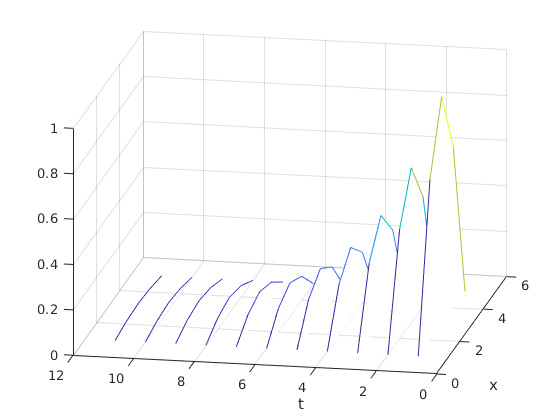
\includegraphics[width=0.305\linewidth]{png/N5}
  }
  \hfill
  \subfigure[$N = 11$]{
    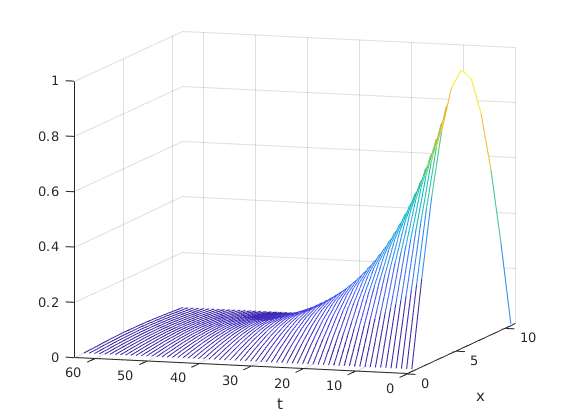
\includegraphics[width=0.305\linewidth]{png/N11}
  }
  \hfill
  \subfigure[$N = 21$]{
    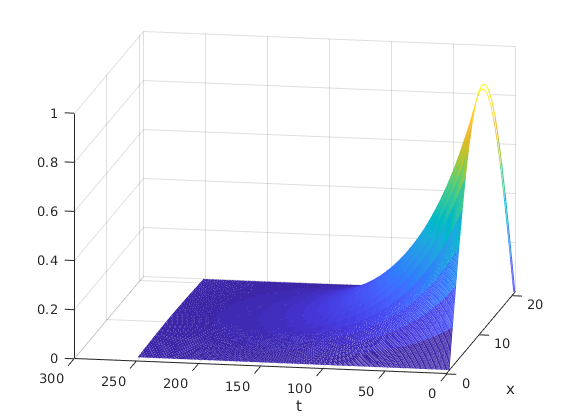
\includegraphics[width=0.305\linewidth]{png/N21}
  }
\end{figure}
Compare with the explicit scheme,
we find that the above implicit scheme is unconditionally stable,
i.e.,
we don't need the restriction $\Delta t = \mathcal{O}(\Delta x^2)$
to ensure convergence.
\end{sol}
%%% Local Variables:
%%% mode: latex
%%% TeX-master: "../hw5"
%%% End:
